\section{Missionen}
\label{sec:module.Missionen}

Missionen sind das Herzst�ck unserer Arbeit. Eine Mission dauert �ber mehrere Spielz�ge und berechnet f�r jede teilnehmende Ameise welches ihr n�chster Move ist. Nachfolgende Darstellung zeigt, dass alle Missionen von der abstrakten BaseMission abstammen und die BaseMission das Interface Mission implementiert. Die Lebensdauer einer Mission h�ngt davon ab, ob sie ihr Ziel erreicht oder ob sie schon f�hrer abgebrochen werden muss. Ziel und Abbruchbedingungen sind je nach Mission unterschiedlich und werden im jeweiligen Abschnitt erkl�rt.

\begin{figure}[H]
\centering
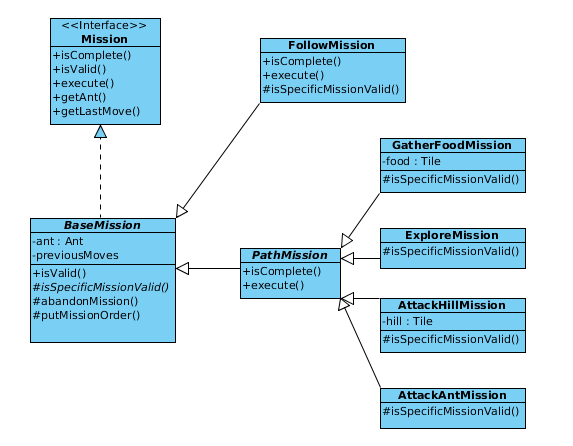
\includegraphics[width=0.9\textwidth]{91_bilder/Missions}
\caption{Missionen und ihre Hierarchie}
\label{fig:missions}
\end{figure}


\subsection{BaseMission}
\label{subsec:module.Mission.BaseMission}

Diese Klasse hat zwei Aufgaben, erstens Implementiert sie die von Interface Mission vorgegebene Methoden und zweitens stellt sie Funktionen zur Verf�gung die von spezifischen Missionen verwendet werden. Die wichtigsten sind hier mit Erkl�rung aufgelistet.

\begin{itemize}
	\item  \textbf{abandonMission():} Abbrechen der Mission
	\item  \textbf{addAnt():} Ameise der Mission hinzuf�gen, in der Population als besch�ftigt markieren.
	\item  \textbf{doAnyMove(Ant a):} F�r die mitgegebene Ameise irgendein Zug in eine der vier Richtung bestimmen.
	\item  \textbf{doMoveInDirection(Ant ant, Tile target): Ein Zug in eine bestimmte Richtung bestimmen.}
	\item  \textbf{gatherAnts(...):} Ameisen f�r die Mission rekrutieren. Anzahl Ameisen wird als Parameter mitgegeben. }
	\item  \textbf{moveToNextTileOnPath(Ant a):} Bewegt die Ameise ein Pfadst�ck weiter auf dem, der Ameisen zugewiesen, Pfad.}
	\item  \textbf{putMissionOrder(...):} Wurde ein Befehl f�r die Ameise gefunden wird er der Klasse Orders (Verwaltung der Befehle) mitgeteilt.}
	\item  \textbf{releaseAnts(int amount):} Ameisen vo der Mission entlassen. 
	\item  \textbf{checkEnviroment(...):} Mittels Breitensuche wird die Umgebung der Ameise nach eigenen H�gel, gegnerischen H�gel, gegnerischen Ameisen und Futterzellen gescannt. Je nach Mission wird beim Fund eines solchen Objekt die Mission abgebrochen, oder die Ameise von der Mission entlassen.
\end{itemize}
\\
\\
Nachfolgend werden die spezifischen Missionen erl�utert. Tabellearisch werden die Eigenschaften der Missionen aufgelistet, danach folgen detailiierte Infomationen zur Mission.


\subsection{PathMission}
\label{subsec:module.Mission.PathMission}

Precondition: -\\
Creator: (Ersteller): CombatTask, oder ExploreMission\\
Postcondition: Pfad vollst�ndig abgelaufen\\
Max. Ants (Maximale Anzahl Ameisen): 1\\
Max. Missionen: unbegrenzt\\
Valid (G�ltigkeit): siehe ExploreMission bzw. CombatTask\\
Gather Ants (Ameisen rektrutieren): Nicht m�glich\\
Release Ants (Ameisen entlassen): Nicht m�glich\\


\subsection{AttackHillMission}
\label{subsec:module.Mission.AttackHillMission}

Precondition: Gegnerischer H�gel sichtbar\\
Creator: AttackHillsTask\\
Postcondition: Gegnerischer H�gel erobert\\
Max. Ants: unbegrenzt\\
Max. Missionen: Je gegnerischen H�gel eine Mission\\
Valid: solange gegnerischer H�gel nicht zerst�rt ist.\\
Gather Ants: pro Zug max. 5 Ameisen, die im Umkreis von 25 Tiles des gegnerischen H�gel sind.\\
Release Ants: Sicheres Food Tile in der N�he. Eigener H�gel in der N�he der Unterst�ztung braucht. Wenn Mission im Status ControlHill ist werden alle Ameisen entlassen ausser zwei. Diese kontrollieren den H�gel.\\

\subsection{DefendHillMission}
\label{subsec:module.Mission.DefendHillMission}

Precondition: Keine, Mission wird zu Beginn des Spiels erstellt.\\
Creator: DefendHillTask\\
Postcondition: Gegnerischer H�gel ist erobert.\\
Max. Ants: unbegrenzt\\
Max. Missionen: Je eigener H�gel eine Mission\\
Valid: solange eigener H�gel nicht erobert ist.\\
Gather Ants: Mission soll immer mehr Verteidiger haben als Angreifer sich dem H�gel n�hern.\\
Release Ants: Keine Angreifer in Sicht, werden die Ameisen (nicht alle) entlassen.\\


\subsection{ExploreMission}
\label{subsec:module.Mission.ExploreMission}

Precondition: - \\
Creator: ExploreTask\\
Postcondition: Definerter Pfad zum Erkunden ist abgelaufen.\\
Max. Ants: 1\\
Max. Missionen: unbegrenzt\\
Valid: Solange Ameise ein g�ltiger Pfad hat.\\
Gather Ants: nicht m�glich\\
Release Ants: nicht m�glich\\

\subsection{GatherFoodMission}
\label{subsec:module.Mission.GatherFoodMission}

Precondition: Keine, Mission wird zu Beginn des Spiels erstellt.\\
Creator: GatherFoodTask\\
Postcondition: diese Mission besteht w�hrend dem ganzen Spiel \\
Max. Ants: unbegrenzt\\
Max. Missionen: 1\\
Valid: immer\\
Gather Ants: siehe Beschreibung\\
Release Ants: siehe Beschreibung\\

\subsection{Verworfene und nicht verwendete Mission}
\label{subsec:implementation.Tasks.StupidMission}

Wie bereits im Kapitel Task erw�hnt war nicht alles programmierte erfolgreich. Hier sind die Missionen aufgelistet die zu den Tasks geh�ren welche verworfen wurden oder nicht verwendet werden.

\begin{itemize}
\item \textbf{SwarmPathMission}
\item \textbf{AttackHillsInFlockMission}
\item \textbf{ConcentrateMission}
\item \textbf{FlockMission}
\end{itemize}

F�r jedes Food-Tile werden in einem definierbaren Radius r die n�chsten Ameisen bestimmt. Danach wird nach aufsteigender Luftliniendistanz mit dem Pfadsuchalgorithmus SIMPLE (s. Abschnitt \ref{subsec:implementation.Pfadsuche.Simple}) oder -- falls dieser keinen Pfad gefunden hat -- mit A* eine passierbare Route gesucht. Wenn ein Pfad existiert, kann mit der Ameise und dem Food-Tile eine GatherFoodMission erstellt werden, welche die Ameise zum Food-Tile f�hrt. Zu jedem Food-Tile wird immer nur eine Ameise geschickt.
